\chapter{Goals and Use Cases}
\label{ch:Goals and Use Cases}

In this chapter, we discuss the intended goals of the project and list some use cases.

\section{Goals}

\paragraph{}
The goal of the project is to develop a software suite which facilitates interoperability between MANO frameworks, thereby enabling management of a network service across multi-vendor environments. To achieve this, we're dividing the software suite into 3 individual modules, which are developed in parallel initially and finally be merged. In the following sections, we discuss the individual goals of these modules in detail.

\subsection{Service Descriptor Translator (SDT)}
\paragraph{}

\subsection{Service Descriptor Splitter (SDS)}
\paragraph{}

\subsection{MANO Adaptor (MA)}
\paragraph{}

A key component of a MANO framework is Virtualized Interface Manager (VIM),  which helps in assigning the hardware resources to virtual resources. The MANO framework uses specific adaptors to communicate with their respective VIMs. For instance, Sonata \ref{SecSONATA} MANO framework has adaptors for OpenStack \ref{label} and Kubernetes\ref{label}. However, when there is a spike in the service request beyond the capabilities of a single MANO instance, multiple MANO instances should be instantiated to balance the load. The goal of this module is to build an adaptor that facilitates interaction between different instances of MANO frameworks, thereby exposing the underlying MANO framework's interfaces and enabling monitoring of the underlying service states.

\paragraph{}
Apart from the implementation of MA, we are planning to investigate MANO scalability challenges by answering research questions such as the ones listed below but not limited to.
\begin{itemize}
	\item What is the optimal number of MANO instances in a system?
	\item What is the optimal hierarchical level in a system?
\end{itemize}


\subsection{Integration Of Work Packages}
\paragraph{}


\begin{figure}[h]
	\centering
	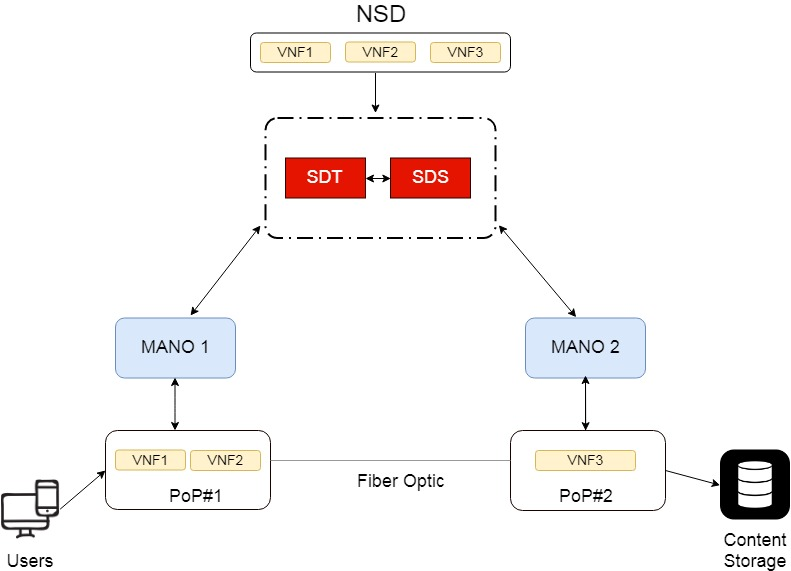
\includegraphics[width=0.7\linewidth]{figures/Structure1}
	\caption{This figure visualizes the structure of first and second modules. }
	\label{fig:structure1}
\end{figure}

\begin{figure}[h]
	\centering
	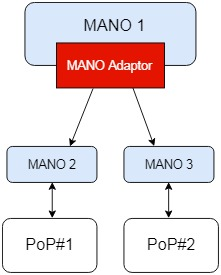
\includegraphics[width=0.3\linewidth]{figures/Structure2}
	\caption{This figure visualizes the structure of third module. }
	\label{fig:structure2}
\end{figure}


\newpage
\section{Use Cases}

\subsection{Cross-MANO Framework Interaction}
\paragraph{}

The MANO frameworks used by every network service provider varies from one another. NSD translation enables the deployment of network services that is in accordance with the intended framework.

For instance: Consider two Network Service Operators using different MANO frameworks. One of them uses Sonata framework \cite{draxler2017sonata} and another operator uses OSM framework \cite{ersue2013etsi}. These frameworks have different NSD schemata(refer \ref{SecSONATA} and \ref{SecOSM}). NSD schemata contains VNFs, virtual links, and VNF forwarding graphs and also describes the deployment of a Network Service. By using a translator, these NSD schemata can be translated to framework-specific schema. With this, operators can deploy and manage Network Services across different MANO implementations.

\subsection{Hierarchical Orchestration}
\paragraph{}
By using the MANO adapter, dynamic instantiation of multiple MANO instances and inter-operability between different MANO frameworks can be achieved. The operator will be able to handle the resources in an efficient manner, as one MANO framework can manage a limited number of service requests, operators can explore options to include additional MANO instances under the existing MANO instance to mitigate the traffic load on a single instance. The resources can be provisioned based on the number of requests. This helps the operator in extending their profitability.
\newpage
\textbf{Actors} : The Network Service Providers who would use features of SCrAMbLE.

\begin{figure} [h]
	\centering
	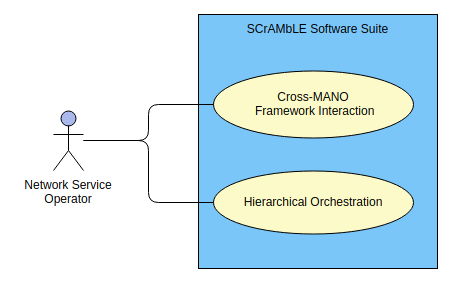
\includegraphics[width=1.0\linewidth]{figures/use-case}
	\caption{Use Case Diagram}
	\label{fig:use-case}
\end{figure}





